\documentclass[UTF8]{ctexart}

\usepackage{tikz}
% Optional PGF libraries
\usepackage{pgflibraryarrows}
\usepackage{pgflibrarysnakes}

\begin{document}

\tableofcontents

\newpage

\section{基础图形}

\begin{center}
	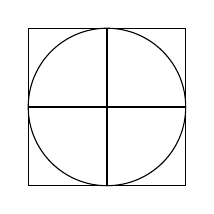
\begin{tikzpicture}
		\draw (-1,-1) rectangle (1,1);
		\draw (0,0) circle (1);
		\draw (0,0) -- (0,1);
		\draw (0,0) -- (1,0);
		\draw (0,0) -- (0,-1);
		\draw (0,0) -- (-1,0);
	\end{tikzpicture}
\end{center}

\newpage

\section{散点图}

\begin{center}
	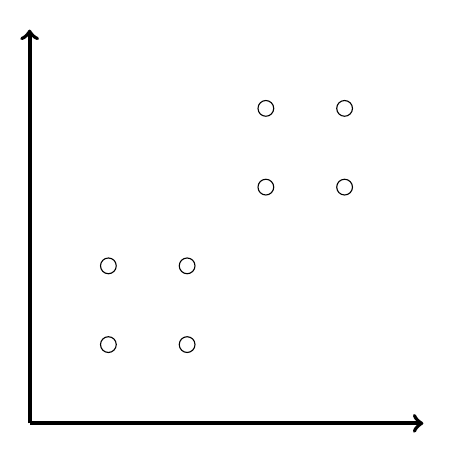
\begin{tikzpicture}
		\def \r {0.1}
		\draw[line width=0.05cm,->] (0,0) -- (0,5);
		\draw[line width=0.05cm,->] (0,0) -- (5,0);
		\draw (1,1) circle (\r);
		\draw (1,2) circle (\r);
		\draw (2,1) circle (\r);
		\draw (2,2) circle (\r);
		\draw (3,3) circle (\r);
		\draw (3,4) circle (\r);
		\draw (4,3) circle (\r);
		\draw (4,4) circle (\r);
	\end{tikzpicture}
\end{center}

\newcommand{\MyThreeDnode}[5]{
		\filldraw[fill=#4, draw=black] (#1 + #3, #2 + #3) circle (#5);
		\draw[dashed] (#1,#2) -- (#1+#3, #2+#3);
		\draw[dashed] (0  ,#2) -- (0+#3,   #2+#3);
		\draw[dashed] (#1,0  ) -- (#1+#3, 0+#3);
		\draw[dashed] (#1,#2) -- (0,  #2);
		\draw[dashed] (#1,#2) -- (#1,0);
		\draw[dashed] (#1 + #3, #2+#3) -- (0  + #3,  #2+ #3);
		\draw[dashed] (#1 + #3, #2+#3) -- (#1+ #3,  0  + #3);
		\draw[dashed] (#1 + #3, 0. +#3) -- (0  + #3,  0  + #3);
		\draw[dashed] (0   + #3, #2+#3) -- (0  + #3,  0  + #3);
}

\begin{center}
	\begin{tikzpicture}
		\draw[line width=0.05cm,->,color=black!50] (0,0) -- (12,0);
		\draw[line width=0.05cm,->,color=black!50] (0,0) -- (0,10);
		\draw[line width=0.05cm,->,color=black!50,dashed] (0,0) -- (7.07,7.07);
		\MyThreeDnode{4}{2}{1.5811}{green!50}{0.2};
		\MyThreeDnode{10}{5}{1}{green!50}{0.2};
		\MyThreeDnode{5}{8}{1.8708}{green!50}{0.2};
		\MyThreeDnode{1}{1}{0.707}{red!50}{0.2};
		\MyThreeDnode{2}{3}{1}{red!50}{0.2};
		\MyThreeDnode{3}{6}{2.1213}{red!50}{0.2};
		\MyThreeDnode{11}{9}{1}{blue!50}{0.2};
		\MyThreeDnode{1}{4}{1.7321}{blue!50}{0.2};
		\MyThreeDnode{9}{1}{1.8708}{blue!50}{0.2};
		\MyThreeDnode{5}{6}{1.8708}{blue!50}{0.2};
	\end{tikzpicture}
\end{center}\par

\end{document}





























